
\begin{figure}[H]
  \centering
  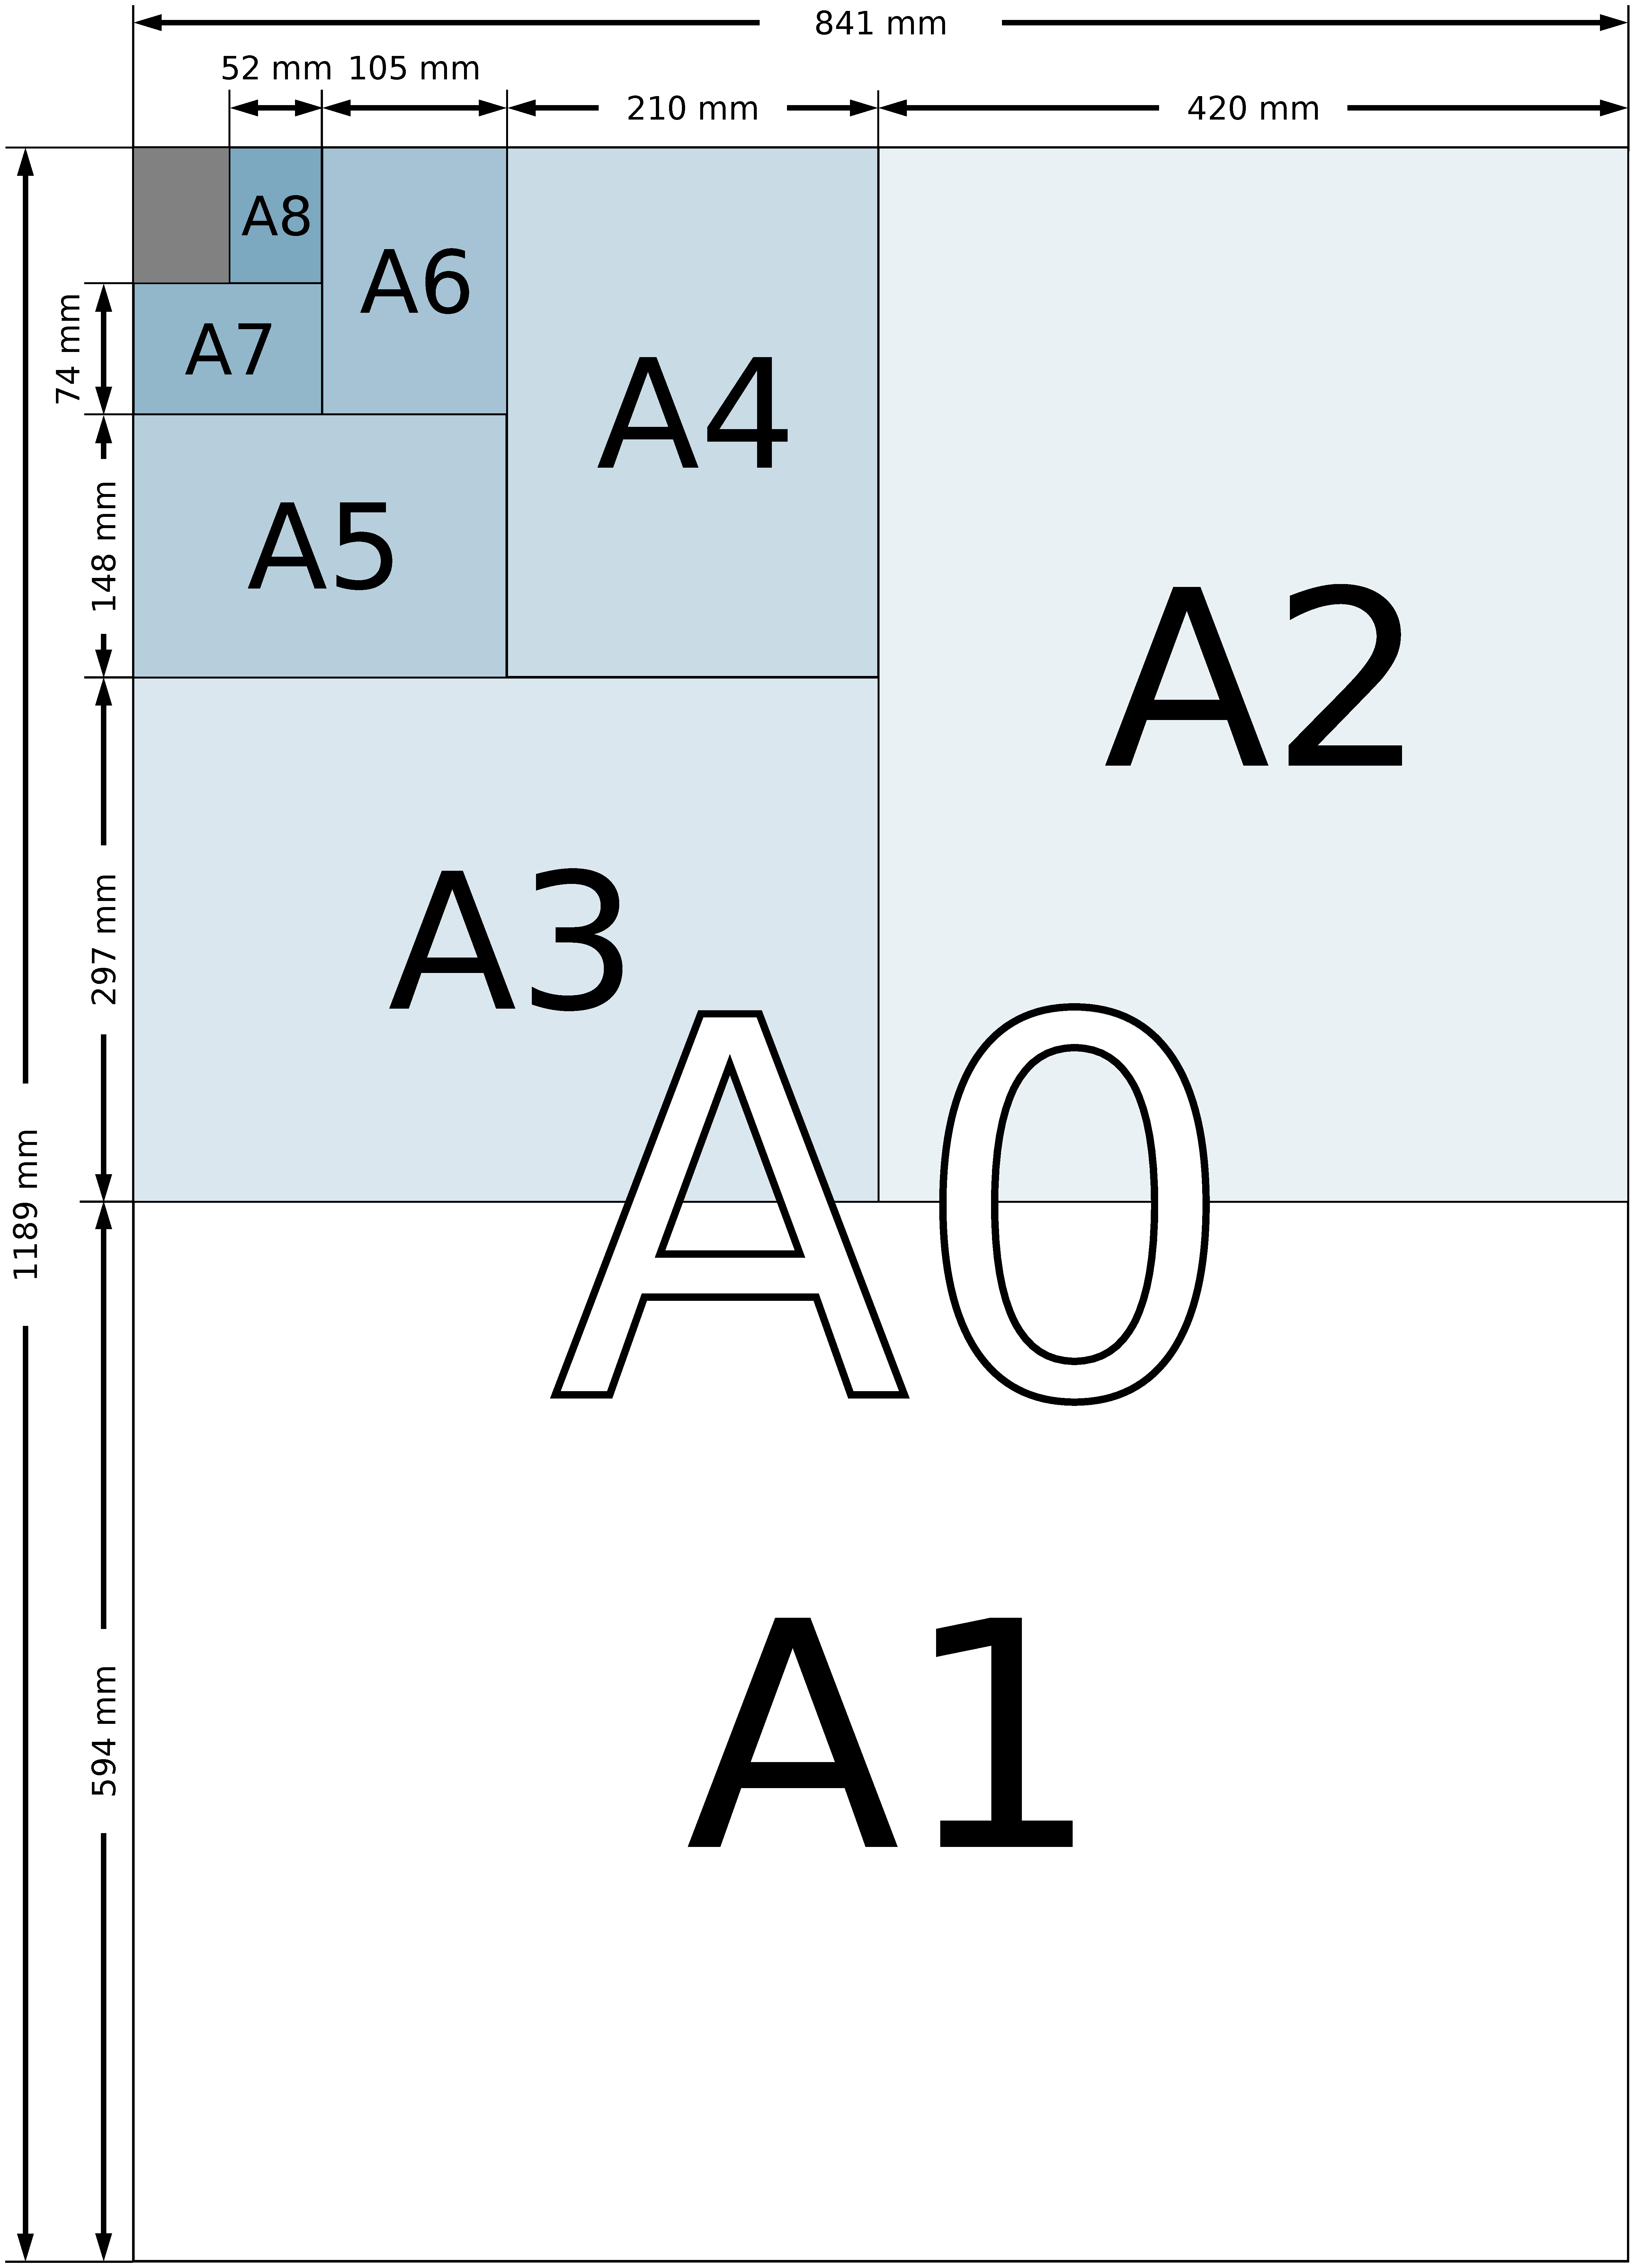
\includegraphics[angle=270,origin=c,width=0.8\textwidth]{includes/A-paper-eps}
\end{figure}

\section*{Introduction}
Understanding the properties of arithmetic and geometric sequences are essential for quantifying the world, and for computing in general. In this paper, I will investigate the different sizes of ISO 216 standard A-series paper, and quantify their properties using my knowledge of sequences.

\section*{The Properties of ISO 216 A-Series Paper}
Let us begin by quantifying the properties of ISO 216 A-series paper (henceforth referred to as A-paper). It is given that the largest A-paper size, $A_{0}$, has a total area of \SI{1}{\metre\squared}. Likewise, we know that each successive smaller paper is the previous paper folded in half.

\subsection*{Formalizing the Area}
We can formalize this property as the following geometric sequence:

\begin{align*}
  a_{n} &= a \times r^{n - 1} \\
  A_{n} &= A \times \left(\frac{1}{2}\right)^{n -1} \\
        &= 2^{-n}
\end{align*}

\noindent
By plugging in the the numbers, it is trivial to generate a table of area for each successive A-series paper:

\begin{table}[h]
  \centering\makegapedcells
    \begin{tabular}{@{}lcl@{}}
    \toprule
    $n$ & Area (fractional \si{\meter\squared}) & Area (decimal \si{\meter\squared}) \\ \midrule
    $0$ & $1$               & $1$              \\
    $1$ & $\frac{1}{2}$     & $0.5$            \\
    $2$ & $\frac{1}{4}$     & $0.25$           \\
    $3$ & $\frac{1}{8}$     & $0.125$          \\
    $4$ & $\frac{1}{16}$    & $0.0625$         \\
    $5$ & $\frac{1}{32}$    & $0.03125$        \\
    $6$ & $\frac{1}{64}$    & $0.015625$       \\ \bottomrule
  \end{tabular}
  \caption{List of A-series paper areas for $0 \geq n \leq 6$}
  \label{tab:area}
\end{table}

\subsection*{Formalizing the Length and Width}
The geometric sequence behind the area of the A-series paper is trivial to discover, but what about the length and width of the paper for a given $n$ in $A_{n}$? Let us begin first by listing the sequence of dimensions for both the length $L_{n}$ and the width $W_{n}$ of $A_{n}$. In order to work with exact values, we will use variables for the starting values rather than their decimal approximations.

\[
  \begin{array}{*{8}{l@{\ }}}
    L_{n} = & L_{0}, & \frac{L_0}{2}, & \frac{L_{0}}{2}, & \frac{L_{0}}{4}, & \frac{L_{0}}{4}, & \frac{L_{0}}{8}, & \frac{L_{0}}{8}, \\[\jot]
    W_{n} = & W_{0}, &         W_{0}, & \frac{W_{0}}{2}, & \frac{W_{0}}{2}, & \frac{W_{0}}{4}, & \frac{W_{0}}{4}, & \frac{W_{0}}{8},
  \end{array}
\]

\subsection*{The Scaling Factor of Conversions}
